\documentclass{article}

% content/resources/templates/preamble.tex
\usepackage[margin=0.6in]{geometry}
\author{Milav Dabgar}
\usepackage{amsmath,amssymb,amsthm}
\usepackage{booktabs}
\usepackage{multirow}
\usepackage{xcolor}
\usepackage{tcolorbox}
\tcbuselibrary{breakable,skins}
\usepackage[colorlinks=true,linkcolor=blue]{hyperref}
\usepackage{titlesec}
\usepackage{enumitem}
\usepackage{tikz}
\usepackage{pgfplots}
\usepackage{circuitikz}
\usepackage[version=4]{mhchem}
\usepackage{longtable}
\usepackage{array}
\usepackage{float}
\usepackage{caption}
\usepackage{listings}

\lstset{
  basicstyle=\small\ttfamily,
  breaklines=true,
  breakatwhitespace=false,
  postbreak=\mbox{\textcolor{red}{$\hookrightarrow$}\space},
  float=false,
  numbers=left,
  numberstyle=\tiny\color{gray},
  numbersep=10pt,
  xleftmargin=2em,
  keywordstyle=\color{blue},
  commentstyle=\color{green!60!black},
  stringstyle=\color{purple},
  backgroundcolor=\color{gray!5},
  showstringspaces=false,
  tabsize=2,
  captionpos=b,
  keepspaces=true,
  columns=flexible
}

\pgfplotsset{compat=1.18}
\usetikzlibrary{shapes,arrows,positioning,calc,patterns,decorations.pathmorphing,decorations.markings,arrows.meta}

% Color scheme
\definecolor{headcolor}{RGB}{0,102,204}
\definecolor{keycolor}{RGB}{220,20,60}
\definecolor{solutioncolor}{RGB}{34,139,34}
\definecolor{mnemoniccolor}{RGB}{148,0,211}
\definecolor{codecolor}{RGB}{0,0,100}

% Spacing
\setlength{\parskip}{3pt}
\setlist[itemize]{nosep}
\setlist[enumerate]{nosep}

% Title formatting
\titleformat{\section}{\Large\bfseries\color{headcolor}}{\thesection}{1em}{}
\titleformat{\subsection}{\large\bfseries\color{headcolor}}{\thesubsection}{1em}{}

% Pandoc tightlist compatibility
\providecommand{\tightlist}{%
  \setlength{\itemsep}{0pt}\setlength{\parskip}{0pt}}

% Pandoc longtable compatibility
\newcounter{none}
\def\thenone{}


% content/resources/templates/english-boxes.tex

% Custom environments
\newtcolorbox{solutionbox}{
 breakable,
 enhanced,
 colback=solutioncolor!5!white,
 colframe=solutioncolor!75!black,
 fonttitle=\bfseries,
 title=Solution
}

\newtcolorbox{solutionboxnobreak}{
 colback=solutioncolor!5!white,
 colframe=solutioncolor!75!black,
 fonttitle=\bfseries,
 title=Solution
}

\newtcolorbox{keyformula}{
 breakable,
 enhanced,
 colback=keycolor!5!white,
 colframe=keycolor!75!black,
 fonttitle=\bfseries,
 title=Key Formula
}

\newtcolorbox{mnemonicboxenv}{
 breakable,
 enhanced,
 colback=mnemoniccolor!5!white,
 colframe=mnemoniccolor!75!black,
 fonttitle=\bfseries,
 title=Mnemonic
}

\newcommand{\mnemonicbox}[1]{%
  \begin{mnemonicboxenv}
    #1
  \end{mnemonicboxenv}
}


% Custom commands for GTU solutions
% This file defines semantic commands for consistent formatting

% Question command with automatic formatting
\newcommand{\question}[2]{%
  \section*{Question #1}%
  \textbf{#2}%
}

% OR question variant
\newcommand{\questionor}[2]{%
  \section*{Question #1 OR}%
  \textbf{#2}%
}

% Proper table environment with caption
\newenvironment{answertable}[1]{%
  \begin{table}[htbp]
  \centering
  \caption{#1}
}{%
  \end{table}
}

% Proper figure environment for diagrams
\newenvironment{answerdiagram}[1]{%
  \begin{figure}[htbp]
  \centering
  \caption{#1}
}{%
  \end{figure}
}

% Semantic markup for key terms
\newcommand{\keyword}[1]{\textbf{#1}}
\newcommand{\code}[1]{\texttt{#1}}
\newcommand{\classname}[1]{\texttt{#1}}
\newcommand{\methodname}[1]{\texttt{#1}}

% Proper quotation marks
\newcommand{\mnemonic}[1]{``#1''}


\title{Industrial Electronics (4331103) - Summer 2023 Solution}
\date{July 21, 2023}

\begin{document}
\maketitle

\questionmarks{1(a)}{3}{Draw and Explain the V-I Characteristics of TRIAC.}

\begin{solutionbox}

TRIAC (Triode for Alternating Current) is a bidirectional three-terminal semiconductor device that can conduct current in either direction when triggered.

\textbf{Diagram:}

\begin{center}
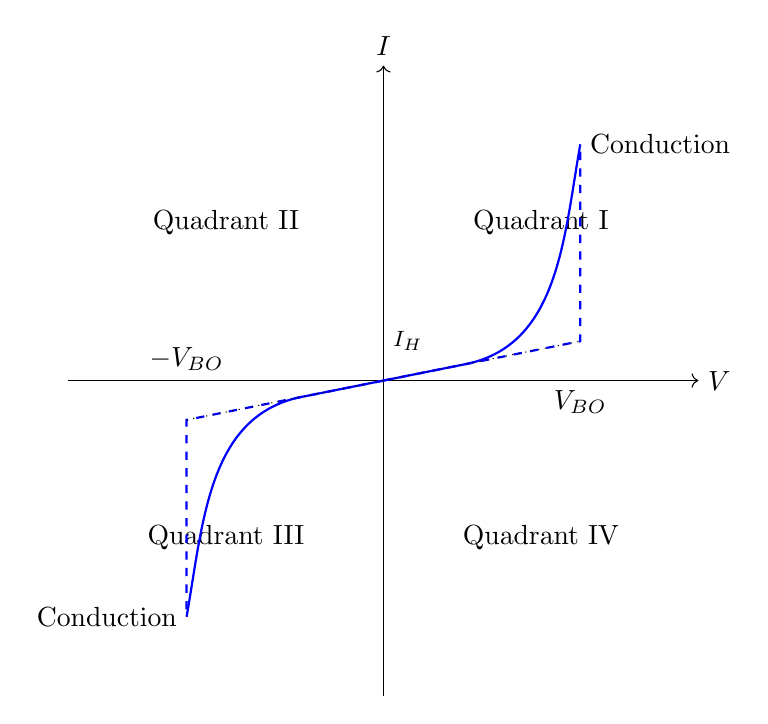
\begin{tikzpicture}
    % Axes
    \draw[->] (-4,0) -- (4,0) node[right] {$V$};
    \draw[->] (0,-4) -- (0,4) node[above] {$I$};
    
    % Quadrant Labels
    \node at (2,2) {Quadrant I};
    \node at (-2,2) {Quadrant II};
    \node at (-2,-2) {Quadrant III};
    \node at (2,-2) {Quadrant IV};
    
    % Curve in Q1
    \draw[thick, blue] (0,0) -- (1,0.2) to[out=10,in=260] (2.5,3);
    \draw[thick, blue, dashed] (0,0) -- (2.5,0.5) -- (2.5,3); % Leakage and breakdown
    \node[right] at (2.5,3) {Conduction};
    \node[below] at (2.5,0) {$V_{BO}$};
    
    % Curve in Q3
    \draw[thick, blue] (0,0) -- (-1,-0.2) to[out=190,in=80] (-2.5,-3);
    \draw[thick, blue, dashed] (0,0) -- (-2.5,-0.5) -- (-2.5,-3);
    \node[left] at (-2.5,-3) {Conduction};
    \node[above] at (-2.5,0) {$-V_{BO}$};
    
    % Holding Current
    \draw[dotted] (-2.5, -0.5) -- (2.5, 0.5);
    \node[right, font=\footnotesize] at (0, 0.5) {$I_H$};

\end{tikzpicture}
\captionof{figure}{V-I Characteristics of TRIAC}
\end{center}

\begin{itemize}
    \item \keyword{Bidirectional operation}: TRIAC conducts in both directions (positive and negative half cycles)
    \item \keyword{Quadrant operation}: Functions in all four quadrants based on polarity of MT2 and gate
    \item \keyword{Triggering voltage}: Breakdown occurs at $\pm V_{BO}$ in either direction
    \item \keyword{Holding current}: Minimum current to maintain conduction
\end{itemize}

\end{solutionbox}
\mnemonicbox{Two Rectifiers In A Case}

\questionmarks{1(b)}{4}{Explain working of SCR using two transistor analogy.}

\begin{solutionbox}

SCR (Silicon Controlled Rectifier) can be represented as interconnected PNP and NPN transistors.

\textbf{Diagram:}

\begin{center}
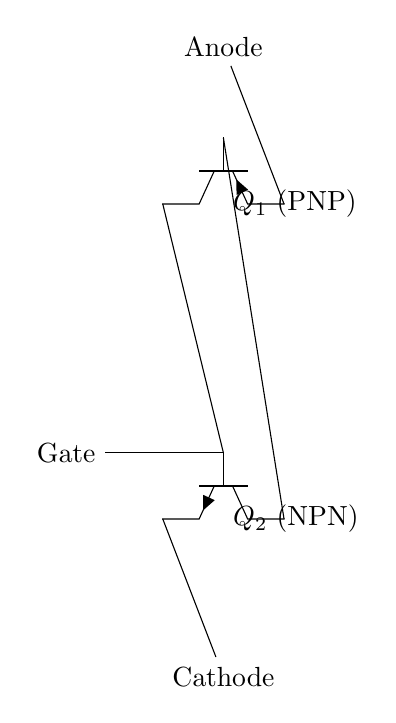
\begin{tikzpicture}[gtu block/.style={draw, rectangle, minimum width=2cm, minimum height=1cm, align=center}]
    % Transistors representation with blocks (simplified for analogy) or circuit symbols
    % Using circuit symbols is better for analogy
    \node (anode) at (0,4) {Anode};
    \node (cathode) at (0,-4) {Cathode};
    
    % PNP Transistor Q1
    \draw (0,2) node[pnp, rotate=-90] (Q1) {};
    \node[right] at (Q1) {$Q_1$ (PNP)};
    
    % NPN Transistor Q2
    \draw (0,-2) node[npn, rotate=-90] (Q2) {};
    \node[right] at (Q2) {$Q_2$ (NPN)};
    
    % Connections
    \draw (anode) -- (Q1.E);
    \draw (Q1.C) -- (Q2.B);
    \draw (Q2.C) -- (Q1.B); % Feedback loop
    \draw (Q2.E) -- (cathode);
    
    % Gate
    \draw (Q2.B) -- ++(-1.5,0) node[left] {Gate};

\end{tikzpicture}
\captionof{figure}{Two Transistor Analogy of SCR}
\end{center}

\begin{itemize}
    \item \keyword{Two-transistor structure}: PNP ($Q_1$) and NPN ($Q_2$) connected such that collector of each transistor drives the base of other
    \item \keyword{Regenerative feedback}: Once both transistors start conducting, they keep each other in saturation
    \item \keyword{Triggering}: Applying gate current to $Q_2$ base starts the regenerative process
    \item \keyword{Latching}: Once triggered, SCR remains ON even if gate signal is removed
\end{itemize}

\end{solutionbox}
\mnemonicbox{Pull Neat Path}

\questionmarks{1(c)}{7}{Draw the circuit diagram of photo electric relay using LDR and explain it Working.}

\begin{solutionbox}

A photoelectric relay using LDR (Light Dependent Resistor) is a light-activated switching circuit.

\textbf{Circuit Diagram:}

\begin{center}
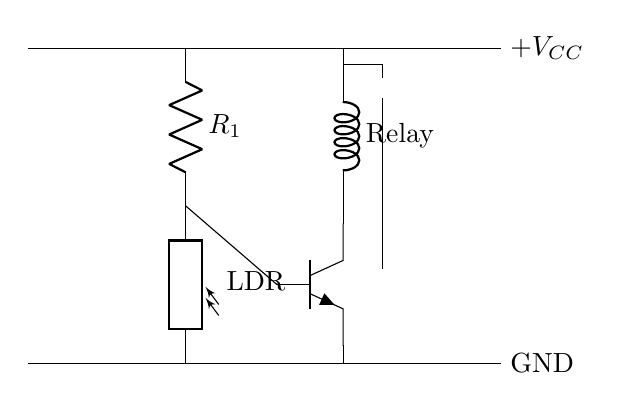
\begin{tikzpicture}
    % Power rails
    \draw (-2,4) -- (4,4) node[right] {$+V_{CC}$};
    \draw (-2,0) -- (4,0) node[right] {GND};
    
    % Potential Divider R1 and LDR
    \draw (0,4) to[R, l=$R_1$] (0,2) to[photoresistor, l=LDR] (0,0);
    
    % Transistor
    \draw (2,1) node[npn] (Q1) {};
    \draw (0,2) -- (Q1.B);
    \draw (Q1.E) -- (2,0);
    
    % Relay Coil
    \draw (2,4) to[L, l=Relay, name=L1] (Q1.C);
    
    % Diode across Relay
    \draw (2.5, 3.5) node[diode, rotate=90] (D1) {}; 
    \draw (2,3.8) -- (2.5, 3.8) -- (D1);
    \draw (2.5, 1.2) -- (D1); % Simplified diode placement

\end{tikzpicture}
\captionof{figure}{Photo Electric Relay Circuit}
\end{center}

\begin{itemize}
    \item \keyword{Light sensing}: LDR resistance decreases in presence of light
    \item \keyword{Transistor operation}: When light falls on LDR, voltage at transistor base changes
    \item \keyword{Relay switching}: Transistor conducts/cuts off based on light, activating/deactivating relay
    \item \keyword{Threshold adjustment}: Potentiometer $R_1$ sets light sensitivity level
    \item \keyword{Applications}: Automatic street lights, burglar alarms, automatic door openers
\end{itemize}

\end{solutionbox}
\mnemonicbox{Light Detects Readily}

\questionmarks{1(c OR)}{7}{Draw the gate pulse trigger circuit using UJT for SCR and explain its working.}

\begin{solutionbox}

UJT (Unijunction Transistor) provides reliable trigger pulses for SCR.

\textbf{Circuit Diagram:}

\begin{center}
\begin{tikzpicture}
    % Supply
    \draw (-1,5) -- (5,5) node[right] {$+V_{CC}$};
    \draw (-1,0) -- (5,0) node[right] {GND};
    
    % RC charging
    \draw (0,5) to[vR, l=$R_1$] (0,2.5) to[C, l=$C$] (0,0);
    
    % UJT
    \draw (2,2.5) node[ujt] (U1) {};
    \draw (0,2.5) -- (U1.E);
    \draw (U1.B2) to[R, l=$R_2$] (2,5);
    \draw (U1.B1) to[R, l=$R_3$] (2,0);
    
    % SCR Triggering
    \draw (4,0) node[thyristor] (S1) {};
    \draw (U1.B1) -- (S1); % Direct or via capacitor/resistor typically
    \draw (2,0.5) -- (3,0.5) -- (3,0.2) node[below] {To SCR Gate};

\end{tikzpicture}
\captionof{figure}{UJT Trigger Circuit for SCR}
\end{center}

\begin{itemize}
    \item \keyword{RC timing}: $R_1$ and $C$ form charging circuit that determines pulse frequency
    \item \keyword{UJT operation}: UJT fires when capacitor voltage reaches peak point voltage
    \item \keyword{Pulse generation}: UJT discharges capacitor producing sharp trigger pulse
    \item \keyword{SCR triggering}: Pulse applied to SCR gate turns it ON at specific points in AC cycle
    \item \keyword{Frequency control}: Adjusting $R_1$ changes pulse frequency for phase control
\end{itemize}

\end{solutionbox}
\mnemonicbox{Uniform Junctions Trigger}

\questionmarks{2(a)}{3}{State Triggering methods of SCR.}

\begin{solutionbox}

\begin{center}
\tablefirsthead{\hline \textbf{Triggering Method} & \textbf{Operating Principle} & \textbf{Advantages} \\ \hline}
\tablehead{\hline \textbf{Triggering Method} & \textbf{Operating Principle} & \textbf{Advantages} \\ \hline}
\tabletail{\hline}
\tablelasttail{\hline}
\begin{tabulary}{\linewidth}{|L|L|L|}
Gate Triggering & Current applied to gate terminal & Most common, precise control \\
Thermal Triggering & Temperature rise causes leakage & Simple, no external circuit \\
Light Triggering & Photons create electron-hole pairs & Electrical isolation, used in LASCRs \\
dv/dt Triggering & Rapid voltage rise causes turn-on & Useful for protection circuits \\
Forward Voltage Triggering & Exceeding breakover voltage & No gate connection needed \\
\end{tabulary}
\captionof{table}{SCR Triggering Methods}
\end{center}

\end{solutionbox}
\mnemonicbox{Good Triggers Let Devices Fire}

\questionmarks{2(b)}{4}{What is Commutation of SCR? Explain class-E commutation.}

\begin{solutionbox}

Commutation is the process of turning OFF an SCR by reducing its anode current below holding current.

\textbf{Class-E Commutation (Complementary Commutation):}

\begin{center}
\begin{tikzpicture}
    % Two SCRs
    \draw (0,4) -- (0,3) node[thyristor] (S1) {} -- (0,0);
    \draw (4,4) -- (4,3) node[thyristor] (S2) {} -- (4,0);
    
    % Commutating Capacitor
    \draw (0,2) -- (2,2) to[C, l=$C$] (2,2) -- (4,2);
    
    % Loads
    \draw (0,0) to[R, l=$R_{L1}$] (0,-2) -- (2,-2);
    \draw (4,0) to[R, l=$R_{L2}$] (4,-2) -- (2,-2);
    \draw (2,-2) -- (2,-3) node[ground] {};
    
    % Supply
    \draw (0,4) -- (2,4) -- (2,5) node[above] {$+V_{DC}$};
    \draw (4,4) -- (2,4);

\end{tikzpicture}
\captionof{figure}{Class-E Commutation Circuit}
\end{center}

\begin{itemize}
    \item \keyword{Complementary switching}: Uses another SCR in opposite half-cycle
    \item \keyword{Natural commutation}: AC source crosses zero, anode current falls below holding current
    \item \keyword{Application}: AC power control circuits, cycloconverters
    \item \keyword{Advantage}: No additional commutation components required
\end{itemize}

\end{solutionbox}
\mnemonicbox{Complementary Elements}

\questionmarks{2(c)}{7}{Draw and explain Snubber Circuit for SCR.}

\begin{solutionbox}

A snubber circuit protects SCR from voltage transients and dv/dt turn-on.

\textbf{Circuit Diagram:}

\begin{center}
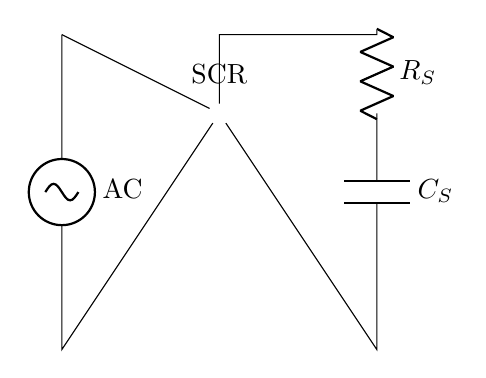
\begin{tikzpicture}
    % SCR
    \draw (0,3) node[thyristor, rotate=-90] (S1) {};
    \node at (0,3.5) {SCR};
    
    % Snubber circuit parallel to SCR
    \draw (S1) -- (0,4) -- (2,4) to[R, l=$R_S$] (2,3) to[C, l=$C_S$] (2,1) -- (2,0) -- (S1);
    
    % Load and Source
    \draw (-2,4) to[sV, l=AC] (-2,0) -- (S1);
    \draw (-2,4) -- (S1);

\end{tikzpicture}
\captionof{figure}{Snubber Circuit for SCR}
\end{center}

\begin{itemize}
    \item \keyword{RC network}: Series resistor ($R_S$) and capacitor ($C_S$) connected across SCR
    \item \keyword{Transient suppression}: Capacitor absorbs voltage spikes that could damage SCR
    \item \keyword{dv/dt protection}: Prevents false triggering due to rapid voltage rise
    \item \keyword{Turn-off assistance}: Helps in commutation by providing alternate current path
    \item \keyword{Component selection}: $C_S$ based on load current, $R_S$ limits discharge current
\end{itemize}

\end{solutionbox}
\mnemonicbox{Safely Neutralizes Unwanted Breakover}

\questionmarks{2(a OR)}{3}{Explain over current protection method of SCR.}

\begin{solutionbox}

\begin{center}

\begin{tabulary}{\linewidth}{|L|L|L|}
\hline \textbf{Protection Method} & \textbf{Working Principle} & \textbf{Applications} \\ \hline
Fuses & Melts when current exceeds rating & Simple, economical protection \\
Circuit Breakers & Trips on overload, can be reset & Reusable protection \\
Current Limiting Reactors & Limits fault current magnitude & Industrial power control \\
Electronic Current Limiting & Senses current and controls gate & Precise protection \\
Crowbar Circuit & Shorts power supply on overload & Protects sensitive loads \\
\end{tabulary}
\captionof{table}{SCR Overcurrent Protection Methods}
\end{center}

\end{solutionbox}
\mnemonicbox{Fault Current Causes Equipment Damage}

\questionmarks{2(b OR)}{4}{Explain the working of opto-SCR.}

\begin{solutionbox}

An opto-SCR (or Light Activated SCR) combines a light source and SCR in an isolated package.

\textbf{Diagram:}

\begin{center}
\begin{tikzpicture}
    % Package Box
    \draw[dashed] (0,0) rectangle (5,3);
    
    % LED input
    \draw (0.5,1.5) to[led, l=LED] (0.5,0.5); 
    \draw (0.5, 2.5) -- (0.5, 1.5);
    \node[left] at (0.5, 2.5) {Anode};
    \node[left] at (0.5, 0.5) {Cathode};

    % Light arrows
    \draw[->, wave] (1.5, 1.5) -- (3, 1.5);
    
    % SCR output
    \draw (4,1.5) node[thyristor, rotate=-90] (S1) {};
    \draw (4, 2.5) -- (S1);
    \draw (4, 0.5) -- (S1);
    \node[right] at (4, 2.5) {Anode};
    \node[right] at (4, 0.5) {Cathode};
    \draw (S1) -- (3.5, 1.5) node[left] {Gate};

\end{tikzpicture}
\captionof{figure}{Opto-SCR Structure}
\end{center}

\begin{itemize}
    \item \keyword{Electrical isolation}: LED optically triggers SCR without electrical connection
    \item \keyword{Noise immunity}: Immune to electrical noise and interference
    \item \keyword{High-voltage isolation}: Separates control and power circuits
    \item \keyword{Applications}: Industrial control, high-voltage switching
\end{itemize}

\end{solutionbox}
\mnemonicbox{Light Activates Silicon Control}

\questionmarks{2(c OR)}{7}{What is force commutation? Explain any two.}

\begin{solutionbox}

Force commutation is artificially turning OFF an SCR by reducing its anode current below holding level.

\textbf{1. Class A Commutation (Self-Commutation):}

\begin{center}
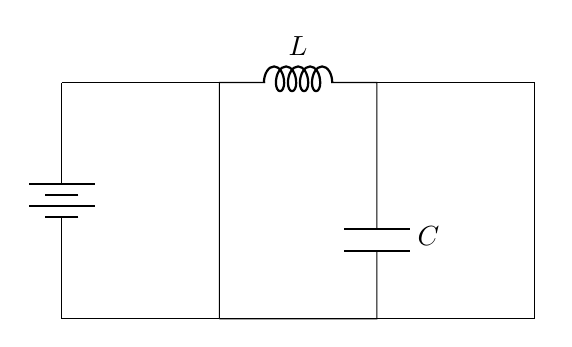
\begin{tikzpicture}
    % Load resonant
    \draw (0,0) -- (0,3) to[L, l=$L$] (2,3) -- (2,2) to[C, l=$C$] (2,0) -- (0,0);
    \draw (2,3) -- (4,3) node[thyristor, rotate=-90] (S1) {} -- (4,0) -- (2,0);
    
    % DC Source
    \draw (-2,3) to[battery] (-2,0) -- (0,0);
    \draw (-2,3) -- (0,3);

\end{tikzpicture}
\captionof{figure}{Class A Commutation}
\end{center}

\begin{itemize}
    \item \keyword{LC resonant circuit}: Parallel L-C across SCR creates oscillations
    \item \keyword{Reverse current}: L-C circuit forces reverse current through SCR
    \item \keyword{Applications}: Inverters, choppers
\end{itemize}

\textbf{2. Class B Commutation (Resonant Pulse Commutation):}

\begin{center}
\begin{tikzpicture}
    % Main SCR path
    \draw (0,4) to[L, l=$L$] (2,4) -- (2,3) node[thyristor] (S1) {} -- (2,0);
    
    % Commutating path
    \draw (2,4) -- (4,4) to[C, l=$C$] (4,2) -- (2,2);
    
    % Source
    \draw (0,4) node[left] {$+V_s$};
    \draw (0,0) node[left] {GND};

\end{tikzpicture}
\captionof{figure}{Class B Commutation}
\end{center}

\begin{itemize}
    \item \keyword{External switch}: Additional SCR or switch triggers commutation
    \item \keyword{Energy storage}: L-C circuit stores energy then reverses SCR current
    \item \keyword{Applications}: DC choppers, controlled rectifiers
\end{itemize}

\end{solutionbox}
\mnemonicbox{Force Circuit Reversal}

\questionmarks{3(a)}{3}{Explain 1-$\phi$ full Wave bridge-controlled rectifier using four diodes \& one SCR.}

\begin{solutionbox}

This circuit combines diodes and an SCR for controlled single-phase full-wave rectification.

\textbf{Circuit Diagram:}

\begin{center}
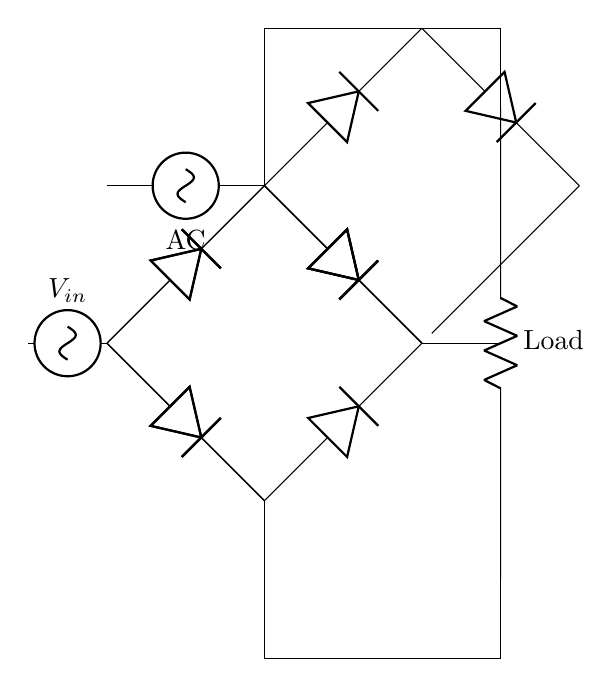
\begin{tikzpicture}
    % Bridge
    \draw (0,2) to[D] (2,4);
    \draw (2,4) to[D] (4,2);
    \draw (0,2) to[D] (2,0);
    \draw (2,0) node[thyristor, rotate=180] (S1) {}; 
    \draw (S1) -- (4,2);
    
    % AC Source
    \draw (0,2) to[sV, l=AC] (-2,2); % Incorrect placement in bridge conceptualization usually 
    % Let's draw standard bridge
    \coordinate (top) at (0,2);
    \coordinate (bottom) at (0,-2);
    \coordinate (left) at (-2,0);
    \coordinate (right) at (2,0);
    
    \draw (left) to[D] (top);
    \draw (top) to[D] (right);
    \draw (left) to[D] (bottom);
    \draw (bottom) node[thyristor, rotate=-90] (S1) {}; % Replacing one diode with SCR? Or SCR at output? 
    % Question says 4 diodes AND 1 SCR. Usually this means a diode bridge feeding an SCR.
    
    % Re-reading: "using four diodes & one SCR". This implies Diode Bridge + Series SCR.
    
    % Diode Bridge
    \draw (-2,0) to[D] (0,2);
    \draw (0,2) to[D] (2,0);
    \draw (-2,0) to[D] (0,-2);
    \draw (0,-2) to[D] (2,0);
    
    % AC Input
    \draw (-3,0) to[sV, l=$V_{in}$] (-2,0);
    \draw (2,0) -- (3,0); 
    
    % SCR in series with Load
    \draw (0,2) -- (0,3) node[thyristor, rotate=-90] (S2) {} -- (0,4);
    \draw (0,-2) -- (0,-4);
    
    % Load
    \draw (3,3) to[R, l=Load] (3,-3);
    \draw (0,4) -| (3,3);
    \draw (0,-4) -| (3,-3);

\end{tikzpicture}
\captionof{figure}{1-$\phi$ Full Wave Rectifier with 4 Diodes and 1 SCR}
\end{center}

\begin{itemize}
    \item \keyword{Bridge configuration}: Four diodes arranged in bridge with one replaced by SCR (or SCR in series)
    \item \keyword{Variable output}: SCR controls conduction angle and thus output voltage
    \item \keyword{Economical design}: Uses only one SCR instead of two or four
    \item \keyword{Efficiency}: Higher than half-wave controlled rectifier
\end{itemize}

\end{solutionbox}
\mnemonicbox{Blend Diodes Smartly}

\questionmarks{3(b)}{4}{What is Chopper? What are its application?}

\begin{solutionbox}

\begin{center}

\begin{tabulary}{\linewidth}{|L|L|}
\hline \textbf{Aspect} & \textbf{Description} \\ \hline
Definition & DC-DC converter that converts fixed DC input to variable DC output \\
Working Principle & Periodically switches DC input ON/OFF at high frequency \\
Types & Step-down (Buck), Step-up (Boost), Buck-Boost, Cuk \\
Control Methods & PWM, Frequency modulation, Current-limit control \\
Applications & DC motor speed control, Battery chargers, UPS, Solar systems, Electric vehicles \\
\end{tabulary}
\captionof{table}{Chopper Basics and Applications}
\end{center}

\end{solutionbox}
\mnemonicbox{Chops Current Perfectly}

\questionmarks{3(c)}{7}{Draw and explain the circuit diagram of static switch using SCR for 1-$\phi$ A.C. Load.}

\begin{solutionbox}

A static switch using SCR provides non-mechanical switching for AC loads.

\textbf{Circuit Diagram:}

\begin{center}
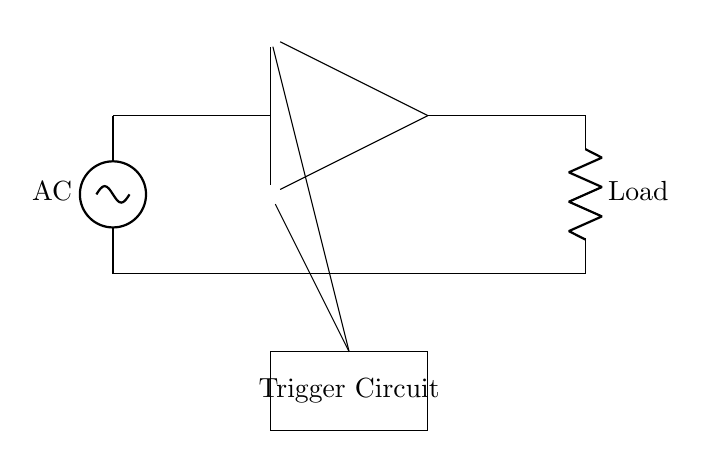
\begin{tikzpicture}
    % Anti-parallel SCRs
    \draw (0,0) -- (2,0);
    \draw (2,1) node[thyristor, rotate=-180] (S1) {};
    \draw (2,-1) node[thyristor] (S2) {};
    
    \draw (2,0) -- (S1);
    \draw (2,0) -- (S2);
    \draw (4,0) -- (S1);
    \draw (4,0) -- (S2);
    
    \draw (4,0) -- (6,0) to[R, l=Load] (6,-2) -- (0,-2) to[sV, l=AC] (0,0);
    
    % Trigger block
    \draw (2,-3) rectangle (4,-4) node[pos=0.5] {Trigger Circuit};
    \draw (S1) -- (3, -3);
    \draw (S2) -- (3, -3);

\end{tikzpicture}
\captionof{figure}{Static AC Switch using SCRs}
\end{center}

\begin{itemize}
    \item \keyword{Antiparallel SCRs}: Two SCRs connected in inverse parallel for bidirectional conduction
    \item \keyword{Gate control}: Properly timed gate signals control power to load
    \item \keyword{Zero-crossing switching}: SCRs naturally turn OFF at zero crossing
    \item \keyword{Applications}: Heater control, motor soft-starting, lighting control
    \item \keyword{Advantages}: No moving parts, silent operation, long life
\end{itemize}

\end{solutionbox}
\mnemonicbox{Solid Switching Technology}

\questionmarks{3(a OR)}{3}{Explain basic principle of DC Chopper.}

\begin{solutionbox}

\begin{center}

\begin{tabulary}{\linewidth}{|L|L|}
\hline \textbf{Component} & \textbf{Function} \\ \hline
Switching Device & SCR, MOSFET, IGBT switches DC at high frequency \\
Control Circuit & Generates PWM gate signals to control ON/OFF time \\
Duty Cycle & Ratio of ON time to total time period determines output \\
Output Filter & Smooths chopped output to reduce ripple \\
Working Principle & Average voltage = Input voltage $\times$ Duty cycle \\
\end{tabulary}
\captionof{table}{DC Chopper Principle}
\end{center}

\end{solutionbox}
\mnemonicbox{Direct Current Control}

\questionmarks{3(b OR)}{4}{Write short note on: Un-interrupted Power Supply (UPS).}

\begin{solutionbox}

UPS provides emergency power when main supply fails.

\textbf{Block Diagram:}

\begin{center}
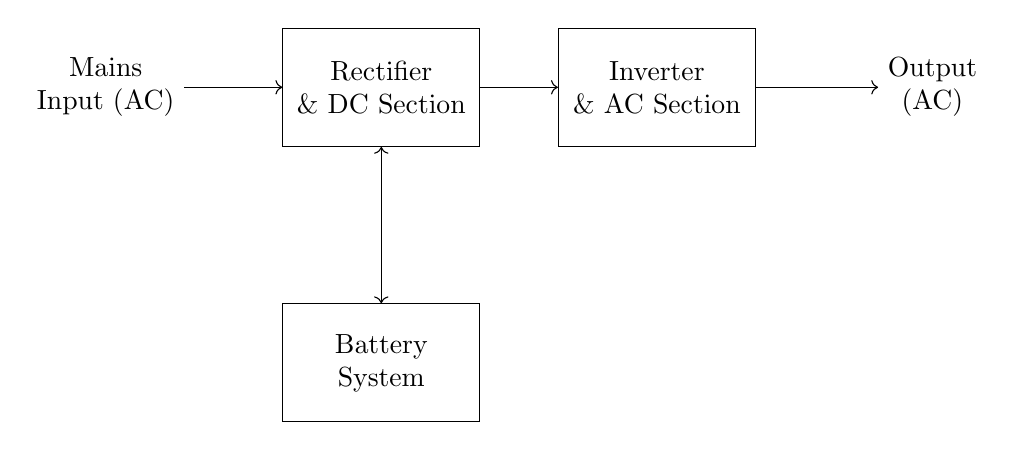
\begin{tikzpicture}[gtu block/.style={draw, rectangle, minimum width=2.5cm, minimum height=1.5cm, align=center}, node distance=3.5cm]
    \node[gtu block] (rect) {Rectifier \\ \& DC Section};
    \node[gtu block, right of=rect] (inv) {Inverter \\ \& AC Section};
    \node[left of=rect, align=center] (input) {Mains \\ Input (AC)};
    \node[right of=inv, align=center] (output) {Output \\ (AC)};
    
    \node[gtu block, below of=rect] (batt) {Battery \\ System};
    
    \draw[->] (input) -- (rect);
    \draw[->] (rect) -- (inv);
    \draw[->] (inv) -- (output);
    \draw[<->] (rect) -- (batt);

\end{tikzpicture}
\captionof{figure}{UPS Block Diagram}
\end{center}

\begin{itemize}
    \item \keyword{Backup power}: Provides continuous power during outages
    \item \keyword{Types}: Online, Offline, Line-interactive UPS
    \item \keyword{Protection}: Against power surges, sags, and frequency variations
    \item \keyword{Applications}: Computers, medical equipment, telecommunications
\end{itemize}

\end{solutionbox}
\mnemonicbox{Uninterrupted Power Securely}

\questionmarks{3(c OR)}{7}{Draw the block diagram of SMPS and explain the function of each block.}

\begin{solutionbox}

Switched-Mode Power Supply converts AC to regulated DC efficiently.

\textbf{Block Diagram:}

\begin{center}
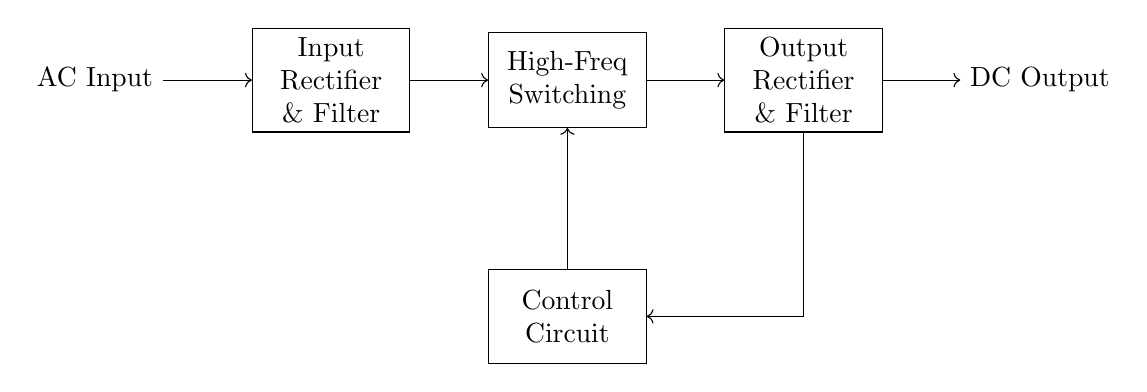
\begin{tikzpicture}[gtu block/.style={draw, rectangle, minimum width=2cm, minimum height=1.2cm, align=center}, auto, node distance=3cm]
    \node[gtu block] (rect1) {Input \\ Rectifier \\ \& Filter};
    \node[gtu block, right of=rect1] (switch) {High-Freq \\ Switching};
    \node[gtu block, right of=switch] (rect2) {Output \\ Rectifier \\ \& Filter};
    \node[right of=rect2] (out) {DC Output};
    \node[left of=rect1] (in) {AC Input};
    
    \node[gtu block, below of=switch] (ctrl) {Control \\ Circuit};
    
    \draw[->] (in) -- (rect1);
    \draw[->] (rect1) -- (switch);
    \draw[->] (switch) -- (rect2);
    \draw[->] (rect2) -- (out);
    
    \draw[->] (rect2) |- (ctrl); % Feedback
    \draw[->] (ctrl) -- (switch); % PWM Control

\end{tikzpicture}
\captionof{figure}{SMPS Block Diagram}
\end{center}

\begin{itemize}
    \item \keyword{Input rectifier}: Converts AC to unregulated DC
    \item \keyword{High-frequency switching}: Converts DC to high-frequency AC using transistors
    \item \keyword{Transformer}: Provides isolation and voltage scaling
    \item \keyword{Output rectifier}: Converts high-frequency AC to DC
    \item \keyword{Filter}: Smooths DC output to reduce ripple
    \item \keyword{Control circuit}: Regulates output through feedback
\end{itemize}

\end{solutionbox}
\mnemonicbox{Switch Mode Power System}

\questionmarks{4(a)}{3}{Draw the circuit diagram using TRIAC for speed control of 1-$\phi$ DC Shunt motor and Explain its working.}

\begin{solutionbox}

TRIAC-based speed control for a DC shunt motor provides efficient variable speed.

\textbf{Circuit Diagram:}

\begin{center}
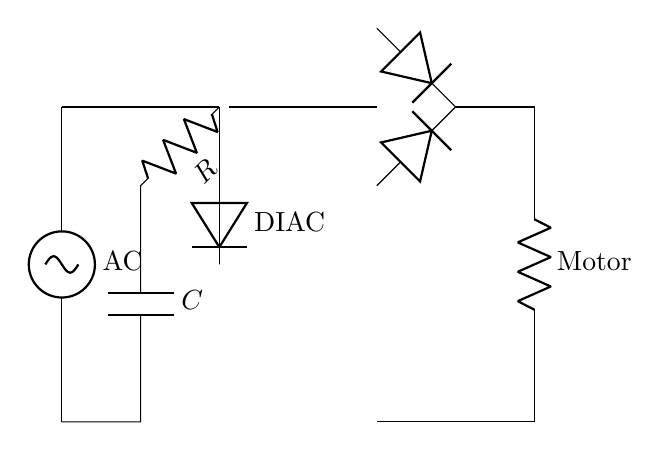
\begin{tikzpicture}
    % AC Source
    \draw (0,4) to[sV, l=AC] (0,0);
    
    % TRIAC control part
    \draw (0,4) -- (2,4);
    \draw (2,4) node[triac, rotate=-90] (TR) {};
    \draw (TR) -- (4,4);
    
    % DIAC Trigger
    \draw (2,4) -- (2,3) to[D, l=DIAC] (2,2) -- (TR);
    
    % Bridge Rectifier
    \draw (4,5) to[D] (5,4);
    \draw (4,3) to[D] (5,4);
    \draw (5,4) -- (6,4) to[R, l=Motor] (6,0) -- (4,0); % Simplified motor load representation
    
    % RC Network
    \draw (2,4) to[R, l=$R$] (1,3) to[C, l=$C$] (1,0) -- (0,0);

\end{tikzpicture}
\captionof{figure}{TRIAC Speed Control for DC Motor}
\end{center}

\begin{itemize}
    \item \keyword{Phase control}: TRIAC varies effective voltage through phase angle control
    \item \keyword{Rectification}: Bridge rectifier converts AC to DC for motor
    \item \keyword{Speed variation}: Motor speed proportional to applied voltage
    \item \keyword{RC timing}: RC network determines firing angle of TRIAC
\end{itemize}

\end{solutionbox}
\mnemonicbox{TRIAC Regulates Speed}

\questionmarks{4(b)}{4}{Draw and explain the circuit diagram four stage sequential timer using IC-556.}

\begin{solutionbox}

IC-556 dual timer can be configured as a multi-stage sequential timer.

\textbf{Circuit Diagram:}

\begin{center}
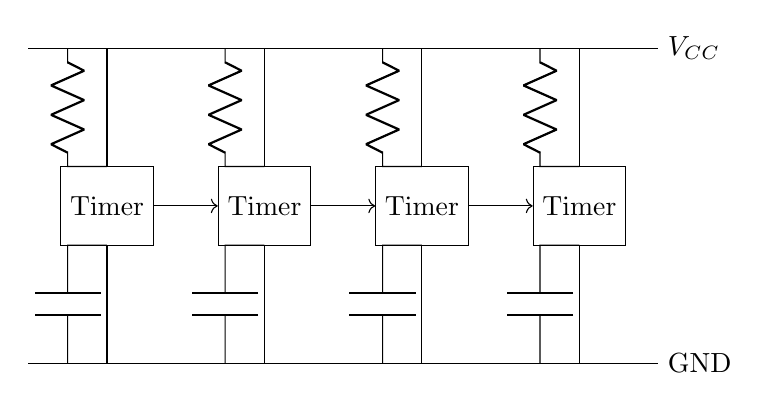
\begin{tikzpicture}
    % Vcc line
    \draw (0,4) -- (8,4) node[right] {$V_{CC}$};
    \draw (0,0) -- (8,0) node[right] {GND};
    
    % 4 Stages abstractly using 555 blocks for clarity as 556 is just 2x555
    \foreach \x in {1, 3, 5, 7} {
        \draw (\x, 2) node[draw, rectangle, minimum size=1cm] (T\x) {Timer};
        \draw (\x, 4) -- (T\x.north);
        \draw (\x, 0) -- (T\x.south);
        \draw (\x, 2.5) -- (\x-0.5, 2.5) to[R] (\x-0.5, 4); % R
        \draw (\x, 1.5) -- (\x-0.5, 1.5) to[C] (\x-0.5, 0); % C
    }
    
    % Cascading
    \draw[->] (T1) -- (T3);
    \draw[->] (T3) -- (T5);
    \draw[->] (T5) -- (T7);

\end{tikzpicture}
\captionof{figure}{Sequential Timer Schematic Concept}
\end{center}

\begin{itemize}
    \item \keyword{Dual timer IC}: IC-556 contains two 555 timer circuits
    \item \keyword{Cascaded configuration}: Output of one stage triggers the next
    \item \keyword{Timing control}: RC time constants determine duration of each stage
    \item \keyword{Applications}: Industrial sequencing, process control, automation
\end{itemize}

\end{solutionbox}
\mnemonicbox{Sequential Steps Timed Precisely}

\questionmarks{4(c)}{7}{Explain induction heating.}

\begin{solutionbox}

Induction heating is a non-contact heating process using electromagnetic induction.

\textbf{Diagram:}

\begin{center}
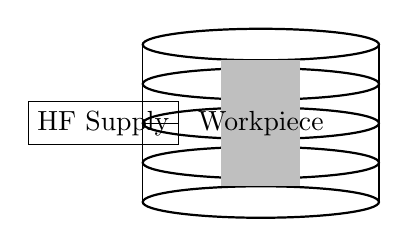
\begin{tikzpicture}
    % Coil
    \foreach \y in {0, 0.5, 1, 1.5, 2} {
        \draw[thick] (0,\y) ellipse (1.5 and 0.2);
    }
    \draw (-1.5, 0) -- (-1.5, 2); % Coil side
    \draw (1.5, 0) -- (1.5, 2); % Coil side
    
    % Workpiece
    \fill[gray!50] (-0.5, 0.2) rectangle (0.5, 1.8);
    \node at (0, 1) {Workpiece};
    
    % Power Supply
    \draw (-2, 1) node[draw] (PS) {HF Supply};
    \draw (PS) -- (-1.5, 1);

\end{tikzpicture}
\captionof{figure}{Induction Heating Setup}
\end{center}

\begin{center}

\begin{tabulary}{\linewidth}{|L|L|}
\hline \textbf{Principle} & \textbf{Description} \\ \hline
Electromagnetic Induction & AC in coil creates alternating magnetic field \\
Eddy Currents & Magnetic field induces currents in workpiece \\
Resistive Heating & Eddy currents generate heat due to material resistance \\
Skin Effect & Current concentrates near surface at high frequencies \\
Applications & Heat treatment, melting, forging, brazing, cooking \\
\end{tabulary}
\captionof{table}{Induction Heating Principles}
\end{center}

\end{solutionbox}
\mnemonicbox{Induced Heating Efficiently}

\questionmarks{4(a OR)}{3}{Draw and explain three stage IC555 timer circuit.}

\begin{solutionbox}

A three-stage timer using IC555 provides sequential timing operations.

\textbf{Circuit Diagram:}

\begin{center}
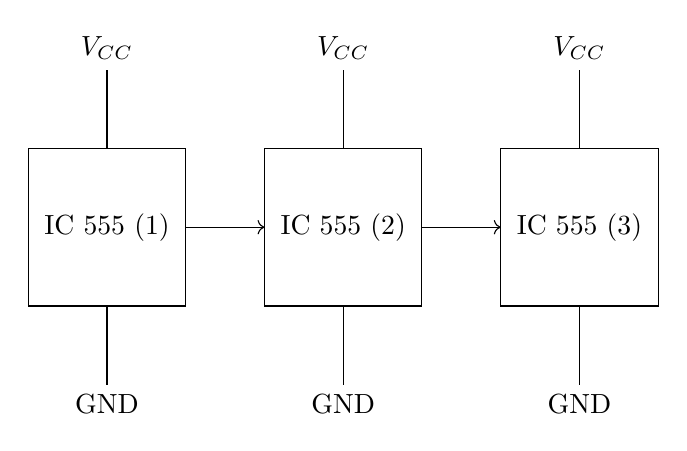
\begin{tikzpicture}
    % Similar to sequential above but 3 stages
    \foreach \x/\n in {0/1, 3/2, 6/3} {
        \draw (\x,0) rectangle (\x+2, 2);
        \node at (\x+1, 1) {IC 555 (\n)};
        \draw (\x+1, 2) -- (\x+1, 3) node[above] {$V_{CC}$};
        \draw (\x+1, 0) -- (\x+1, -1) node[below] {GND};
        
        \ifnum \x<6
            \draw[->] (\x+2, 1) -- (\x+3, 1);
        \fi
    }
\end{tikzpicture}
\captionof{figure}{Three Stage IC555 Timer}
\end{center}

\begin{itemize}
    \item \keyword{Monostable mode}: Each stage operates in monostable mode with fixed time delay
    \item \keyword{Cascaded connection}: Output of first timer triggers second, and so on
    \item \keyword{Timing components}: R-C network determines time delay of each stage
    \item \keyword{Applications}: Automatic sequencing, process timing, industrial control
\end{itemize}

\end{solutionbox}
\mnemonicbox{Time Intervals Created}

\questionmarks{4(b OR)}{4}{Explain the principle of dielectric heating.}

\begin{solutionbox}

\begin{center}

\begin{tabulary}{\linewidth}{|L|L|}
\hline \textbf{Principle} & \textbf{Description} \\ \hline
High-Frequency Electric Field & Material placed between electrodes with RF voltage (1-100 MHz) \\
Molecular Friction & Dipole molecules vibrate/rotate trying to align with alternating field \\
Heat Generation & Internal friction between molecules generates heat uniformly \\
Non-Conductive Materials & Effective for heating non-conductive materials (plastics, wood, food) \\
Applications & Plastic welding, wood drying, food processing (microwave ovens) \\
\end{tabulary}
\captionof{table}{Dielectric Heating Principles}
\end{center}

\end{solutionbox}
\mnemonicbox{Dielectric Energy Heats}

\questionmarks{4(c OR)}{7}{Make comparison between Induction heating and Dielectric heating.}

\begin{solutionbox}

\begin{center}

\begin{tabulary}{\linewidth}{|L|L|L|}
\hline \textbf{Parameter} & \textbf{Induction Heating} & \textbf{Dielectric Heating} \\ \hline
Basic Principle & Electromagnetic induction & High-frequency electric field \\
Suitable Materials & Conductive materials (metals) & Non-conductive materials (plastics, wood) \\
Frequency Range & 1 kHz to 1 MHz & 1 MHz to 1 GHz \\
Heating Mechanism & Eddy currents and hysteresis & Molecular friction (dipole rotation) \\
Heat Distribution & Surface heating (skin effect) & Volumetric (uniform throughout) \\
Efficiency & 80-90\% for magnetic materials & 50-70\% depending on material \\
Applications & Metal melting, forging, heat treatment & Plastic welding, food processing, drying \\
Equipment & Induction coil, work piece & Electrodes, dielectric material \\
\end{tabulary}
\captionof{table}{Comparison of Induction vs Dielectric Heating}
\end{center}

\end{solutionbox}
\mnemonicbox{ICED}

\questionmarks{5(a)}{3}{Explain Construction and working of Universal Motor.}

\begin{solutionbox}

Universal motor operates on both AC and DC power sources.

\textbf{Diagram:}

\begin{center}
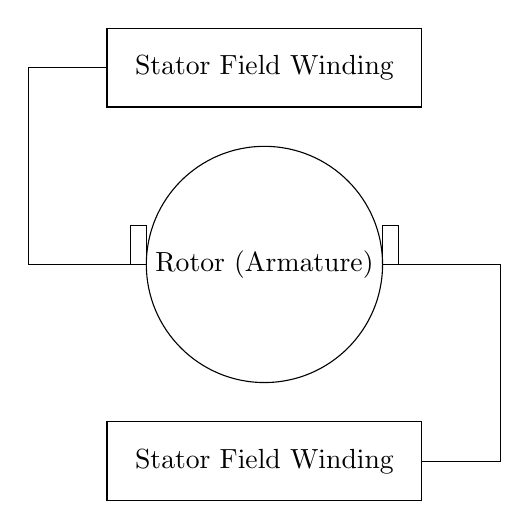
\begin{tikzpicture}
    % Stator
    \draw (-2, 2) rectangle (2, 3) node[pos=0.5] {Stator Field Winding};
    \draw (-2, -3) rectangle (2, -2) node[pos=0.5] {Stator Field Winding};
    
    % Rotor
    \draw (0,0) circle (1.5);
    \node at (0,0) {Rotor (Armature)};
    
    % Brushes
    \draw (-1.7, 0) rectangle (-1.5, 0.5);
    \draw (1.5, 0) rectangle (1.7, 0.5);
    
    % Series connection
    \draw (-2, 2.5) -- (-3, 2.5) -- (-3, 0) -- (-1.7, 0);
    \draw (1.7, 0) -- (3, 0) -- (3, -2.5) -- (2, -2.5);

\end{tikzpicture}
\captionof{figure}{Universal Motor Construction}
\end{center}

\begin{itemize}
    \item \keyword{Series connection}: Field winding in series with armature winding
    \item \keyword{Construction}: Stator with field winding, rotor with commutator and brushes
    \item \keyword{Operating principle}: Same direction torque on both AC and DC
    \item \keyword{Characteristics}: High starting torque, high speed at low load
    \item \keyword{Applications}: Portable tools, household appliances, blenders
\end{itemize}

\end{solutionbox}
\mnemonicbox{Universally Motorized}

\questionmarks{5(b)}{4}{Draw and explain the construction of DC servo motor.}

\begin{solutionbox}

DC servo motor provides precise position or speed control.

\textbf{Diagram:}

\begin{center}
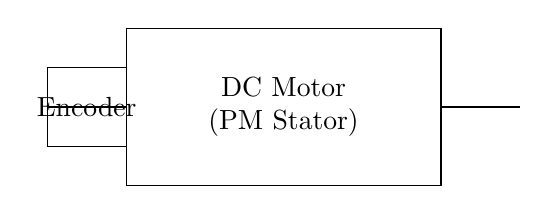
\begin{tikzpicture}
    % Motor Body
    \draw (0,0) rectangle (4,2);
    \node[align=center] at (2,1) {DC Motor \\ (PM Stator)};
    
    % Shaft
    \draw (4,1) -- (5,1);
    
    % Encoder/Feedback
    \draw (-1,0.5) rectangle (0,1.5);
    \node at (-0.5, 1) {Encoder};
    \draw (0,1) -- (-1,1); % Shaft connection to encoder

\end{tikzpicture}
\captionof{figure}{DC Servo Motor}
\end{center}

\begin{itemize}
    \item \keyword{Construction}: Permanent magnet stator, lightweight rotor, feedback device
    \item \keyword{Control system}: Closed-loop control with position/velocity feedback
    \item \keyword{Low inertia}: Allows quick response and precise positioning
    \item \keyword{Applications}: Robotics, CNC machines, positioning systems
    \item \keyword{Features}: High torque-to-inertia ratio, fast response, accuracy
\end{itemize}

\end{solutionbox}
\mnemonicbox{Servo System Control}

\questionmarks{5(c)}{7}{Draw the block diagram of Programmable logic Control (PLC) and explain the Function of each block.}

\begin{solutionbox}

PLC is an industrial digital computer for automation control.

\textbf{Block Diagram:}

\begin{center}
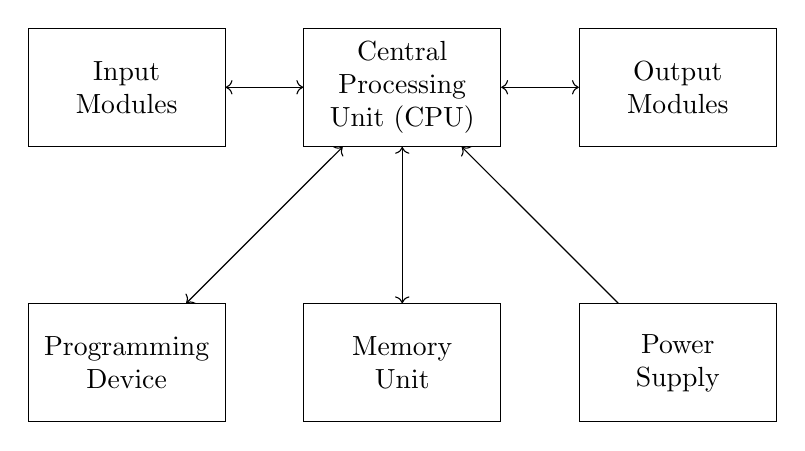
\begin{tikzpicture}[gtu block/.style={draw, rectangle, minimum width=2.5cm, minimum height=1.5cm, align=center}, node distance=3.5cm]
    \node[gtu block] (cpu) {Central \\ Processing \\ Unit (CPU)};
    \node[gtu block, left of=cpu] (in) {Input \\ Modules};
    \node[gtu block, right of=cpu] (out) {Output \\ Modules};
    \node[gtu block, below of=cpu] (mem) {Memory \\ Unit};
    \node[gtu block, below of=in] (prog) {Programming \\ Device};
    \node[gtu block, below of=out] (pwr) {Power \\ Supply};
    
    \draw[<->] (in) -- (cpu);
    \draw[<->] (cpu) -- (out);
    \draw[<->] (cpu) -- (mem);
    \draw[<->] (prog) -- (cpu);
    \draw[->] (pwr) -- (cpu);

\end{tikzpicture}
\captionof{figure}{PLC Block Diagram}
\end{center}

\begin{itemize}
    \item \keyword{CPU}: Executes program, processes I/O data, makes decisions
    \item \keyword{Input modules}: Convert field signals (sensors, switches) to digital signals for CPU
    \item \keyword{Output modules}: Convert CPU commands to actuator signals (motors, valves)
    \item \keyword{Memory unit}: Stores program and data (ROM for OS, RAM for user program)
    \item \keyword{Programming device}: PC or console for program development and monitoring
    \item \keyword{Power supply}: Provides regulated power to PLC components
\end{itemize}

\end{solutionbox}
\mnemonicbox{Programs Logic Completely}

\questionmarks{5(a OR)}{3}{Draw and explain the construction of Stepper motor.}

\begin{solutionbox}

Stepper motor rotates in discrete steps for precise positioning.

\textbf{Diagram:}

\begin{center}
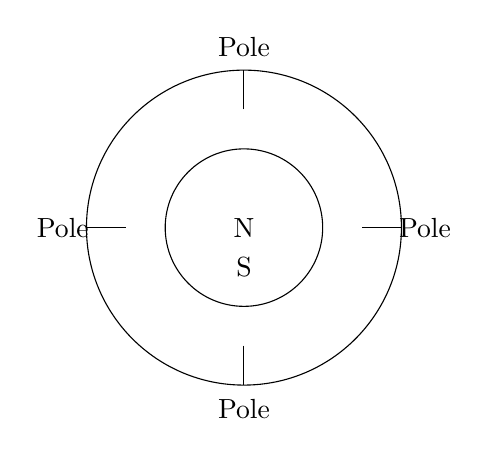
\begin{tikzpicture}
    % Stator
    \draw (0,0) circle (2);
    \foreach \x in {0, 90, 180, 270} {
        \draw (\x:1.5) -- (\x:2); % Poles
        \node at (\x:2.3) {Pole};
    }
    
    % Rotor
    \draw (0,0) circle (1);
    \node at (0,0) {N};
    \node at (0, -0.5) {S};

\end{tikzpicture}
\captionof{figure}{Stepper Motor Construction}
\end{center}

\begin{itemize}
    \item \keyword{Stator}: Contains multiple coil windings (phases)
    \item \keyword{Rotor}: Permanent magnet or variable reluctance type
    \item \keyword{Types}: Permanent magnet, variable reluctance, hybrid
    \item \keyword{Step angle}: Typically 1.8$^{\circ}$ (200 steps/rev) or 0.9$^{\circ}$ (400 steps/rev)
    \item \keyword{Applications}: Printers, disk drives, robotics, CNC machines
\end{itemize}

\end{solutionbox}
\mnemonicbox{Steps Precisely Moved}

\questionmarks{5(b OR)}{4}{Draw explain solid state circuit to control DC shunt Motor Speed.}

\begin{solutionbox}

Solid-state circuit provides efficient and smooth DC motor speed control.

\textbf{Circuit Diagram:}

\begin{center}
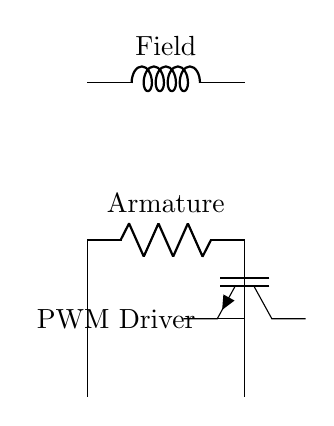
\begin{tikzpicture}
    % Field
    \draw (0,4) to[L, l=Field] (2,4);
    
    % Armature + MOSFET
    \draw (0,2) to[R, l=Armature] (2,2) -- (2,1) node[nigbt, rotate=-90] (Q1) {} -- (2,0); % Using IGBT symbol often for power switch
    \draw (0,2) -- (0,0);
    
    % Gate Drive
    \draw (Q1) -- (1.5, 1) node[left] {PWM Driver};

\end{tikzpicture}
\captionof{figure}{Solid State DC Motor Control}
\end{center}

\begin{itemize}
    \item \keyword{PWM controller}: Generates variable duty cycle pulses to control speed
    \item \keyword{MOSFET driver}: Provides gate drive to power MOSFET
    \item \keyword{Power MOSFET}: Controls current through armature winding
    \item \keyword{Feedback}: Tachogenerator or encoder provides speed feedback
    \item \keyword{Advantages}: Efficient, smooth control, wide speed range
\end{itemize}

\end{solutionbox}
\mnemonicbox{Power With MOSFET}

\questionmarks{5(c OR)}{7}{Explain the Working of VFD (Variable Frequency Drive).}

\begin{solutionbox}

VFD controls AC motor speed by varying frequency and voltage.

\textbf{Block Diagram:}

\begin{center}
\begin{tikzpicture}[gtu block/.style={draw, rectangle, minimum width=2.2cm, minimum height=1.2cm, align=center}, node distance=3cm]
    \node[gtu block] (rect) {Rectifier};
    \node[gtu block, right of=rect] (dc) {DC Link};
    \node[gtu block, right of=dc] (inv) {Inverter};
    \node[right of=inv] (motor) {AC Motor};
    \node[left of=rect] (ac) {AC Main};
    
    \draw[->] (ac) -- (rect);
    \draw[->] (rect) -- (dc);
    \draw[->] (dc) -- (inv);
    \draw[->] (inv) -- (motor);
    
    \node[gtu block, below of=dc] (ctrl) {Control \\ Circuit};
    \draw[->] (ctrl) -- (inv);

\end{tikzpicture}
\captionof{figure}{VFD Block Diagram}
\end{center}

\begin{center}

\begin{tabulary}{\linewidth}{|L|L|}
\hline \textbf{Component} & \textbf{Function} \\ \hline
Rectifier & Converts AC input to DC (diode bridge or active front end) \\
DC Link & Filters DC and stores energy (capacitors, sometimes inductors) \\
Inverter & Converts DC to variable frequency AC (IGBTs with PWM) \\
Control Circuit & Regulates frequency/voltage based on speed requirement \\
Braking Circuit & Dissipates regenerative energy during deceleration \\
\end{tabulary}
\captionof{table}{VFD Components}
\end{center}

\begin{itemize}
    \item \keyword{Speed control}: Motor speed proportional to frequency ($RPM = 120f/P$)
    \item \keyword{Torque control}: Maintains V/f ratio for constant torque
    \item \keyword{Energy savings}: Reduces energy consumption at lower speeds
    \item \keyword{Applications}: Pumps, fans, conveyors, process control
    \item \keyword{Features}: Soft start, overcurrent protection, regenerative braking
\end{itemize}

\end{solutionbox}
\mnemonicbox{Vary Frequency, Drive motor}

\end{document}
